\chapter{Introduction}
\label{chap:introduction}

The proliferation of commodity cloud services poses new challenges and
opportunities for hosting data.  On the one hand, the availability of
professionally-maintained services is a boon to developers, since it lets them
offloads the operational burden of hosting application data.  On the other
hand, it is difficult to leverage these services over long
timescales.  Services can appear and disappear, and service operators can
unilaterally change their APIs, pricing, and trustworthiness.
Over long enough timescales, developers will find themselves continuously
patching their applications to accomodate new service behaviors.

This thesis presents a novel storage architecture, called \emph{wide-area
software-defined storage} (SDS), that helps developers
leverage commodity cloud services without this constant churn.
SDS allows developers to specify their
end-to-end \emph{storage semantics} up front, independently of
both applications and underlying services.  The storage semantics define the
rules for processing reads and writes end-to-end, and reside in an architectural
layer ``on top'' of cloud services but ``beneath'' applications.
This thesis presents SDS as an architecture for implementing these semantics, and
shows how developers can realize the benefits of cloud services without the
long-term risks.

\section{The System-of-Systems Approach}

Applications built on commodity cloud services are systems-of-systems.
A \emph{system-of-systems} is a process that that aggregates the
functionality provided by multiple independent networked processes
in order to solve a problem that none of them could
handle on their own.  The most prominent system-of-systems 
is the Internet, which uses peering agreements and the Border Gateway
Protocol~\cite{bgp} to aggregate the routing logic in
multiple autonomous networks to provide a global end-to-end packet delivery
service.

Networked processes that run in the application layer of the Internet can also
be systems-of-systems.  For example, a university Webmail
application is a system-of-systems that 
aggregates DNS, the world's SMTP servers, campus-hosted
Web servers, and a university-wide identity and authentication
system to grant students and faculty access to their email in their Web browsers
(Figure~\ref{fig:chap1-system-of-systems}).  This example illustrates
how application-layer systems can be combined with other
application-layer systems to build new application-layer systems.

\begin{figure}[h]
   \caption{Webmail is a system-of-systems wide-area application.  In order for
   Alice to receive an email from Bob, her university's DNS and SMTP servers
   must coordinate with the global DNS and SMTP networks, and her university's
   identity service and Webmail servers must coordinate to deliver her mail to
   her Web browser.}
   \centering
   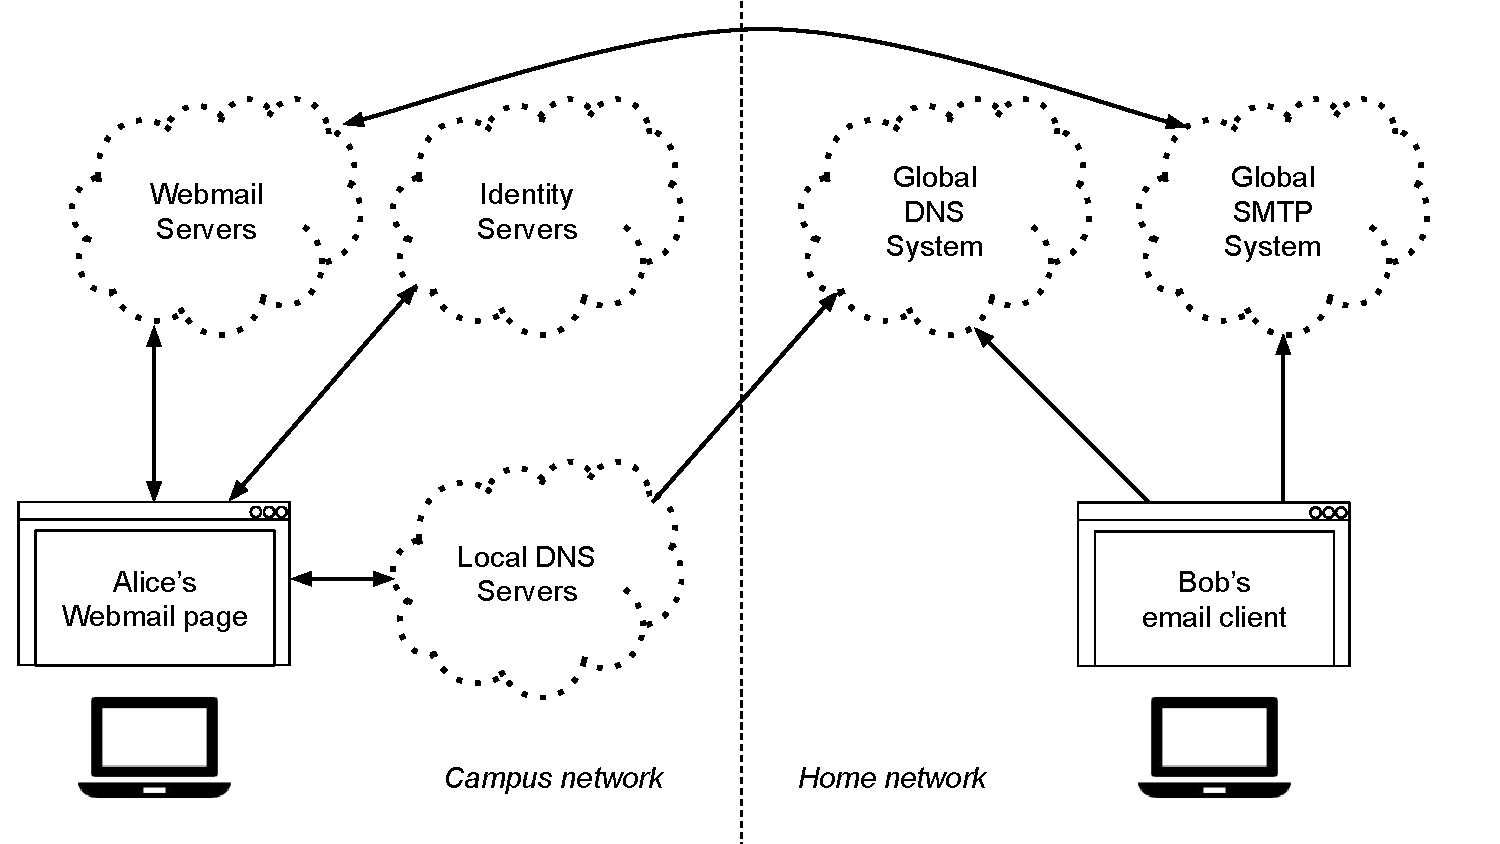
\includegraphics[width=0.9\textwidth,page=1]{figures/dissertation-figures}
   \label{fig:chap1-system-of-systems}
\end{figure}

This thesis is concerned with helping developers build user-facing
system-of-systems applications on top of \emph{cloud storage},
\emph{content distribution networks} (CDNs), and \emph{curated data-sets}.
An application would use cloud storage providers to host
its data, CDNs to accelerate data delivery to readers,
and curated datasets to provide better application value.
For example, an application like OpenStreetMap~\cite{openstreetmap}
would host its users' preferred routes, maps, and historic queries in cloud storage,
use a CDN to cache map data in appropriate geographic regions,
and use public weather data aggregated by NOAA~\cite{noaa} to predict how long a commute may take.

In these applications, developers spend non-trivial amounts of implementation effort
on preserving end-to-end storage semantics.  This is because an application's
storage semantics depend on the semantics of each system it uses.  
In order to build a correct implementation, developers must account for
the semantics of their chosen cloud services in the application's design.
For example, Web application servers must coordinate with downstream CDN nodes to ensure that
clients read fresh data.  As another example, scientific computing clusters
must ensure that only PIs can read sensitive data, and only from within the lab.
In today's system-of-systems applications, these semantics may be interwoven
with the business logic.

% TODO: numbers from e.g. Gartner about the growth of the cloud services market?
Despite the difficulty, the growth of the cloud services market and the proliferation of
applications relying on them demonstrates their promise as system-of-systems
building blocks.  Developers do not have to re-invent the functionality they
provide each time they build a new application.  Developers can instead
simply purchase more service capacity to
handle both their existing and new applications' needs.
This reduces time-to-market, speeds up product iteration,
and lowers the barrier to entry for building new applications.

\subsection{Challenges}

The benefits of building system-of-systems with cloud services are overshadowed
by three challenges.  First, \emph{the underlying services
are unreliable in the long-term}.  They can unilaterally
change their pricing, feature-set, APIs, semantics, availability, and
trustworthiness.  Applications that rely on a service can break without warning
when the service changes its behaviors, and in doing so,
cost developers unforeseeable amounts of time and money.

This unreliability is agreed to in the legal terms of service.  The terms of
service for popular services explicitly state that the operators have the ability to affect unilateral
changes.  For example, Dropbox unilaterally broke its API from version 1 to version
2~\cite{dropbox-v2-api-psa}, and Twitter dropped its API only after non-trivial
applications were built to leverage it~\cite{twitter-api-deprecation-psa}.

The second challenge is that \emph{cloud services are heterogeneous}.
Services that fill similar roles do not offer compatible interfaces or semantics.
Without careful planning, the application can become implicitly coupled to the
services it uses by accidentally relying on undocumented or unacknowledged
semantics.  For example, a service designed to use a single Amazon S3 bucket may implicitly
depend on its sequential consistency, and may not be able to simply switch to
using Box.net (which provides eventual
consistency~\cite{consistency-comparison-cloud-storage}).
This creates unexpectedly high service switching costs, making it
difficult for developers to address service unreliability or move to better
offerrings.

The third challenge has to do with the fact that applications span multiple
organizations.  For the purposes of this thesis, an \emph{organization} is a set of computers that
adhere to a single data-hosting policy for the data they produce.  Example organizations
include a user's personal devices, a corporation's workstations, or a lab's scientific
compute cluster.  The data-hosting policy determines the conditions under which
reads and writes are allowed to occur, and addresses concerns such as access
controls, data availability, data durability, replica placement, and so on.
The user or users of an organization set its data-hosting policy.

Successful system-of-systems applications respect each organization's
data-hosting policies.  For example, email allows each
organization with an SMTP server to control the store-and-forward policies
of email messages that pass through it.  As another example, federated applications
like Mastadon~\cite{mastadon}, IRC~\cite{irc}, and XMPP~\cite{xmpp} allow each
organization to set rules on how users' uploaded data gets stored and relayed.
In these cases, the applications preserve each organization's policies
by making organizations responsible for hosting their data.

The challenge posed to developers when building on cloud services is that
\emph{organizations no longer host their data}.  Data hosting is outsourced
to the services, which puts organizations in a difficult position with
regards to enforcing their policies.  Either an organization \emph{completely trusts} the
cloud services in this capacity, or it does not run the
application at all.

Since each organization makes its own choices about trust in cloud services,
it becomes difficult for developers to respect their specific policies.
Developers either have to forgo certain organizations
as customers, or implement complex application logic to accomodate different
policies.

\section{Wide-area Software-defined Storage}

This thesis addresses these challenges by separating storage semantics from both
cloud services and applications.  The rules for processing reads and writes
from application end-points are placed in a common data-exchanging
layer in-between applications and the cloud services.  A system that
implements this layer is called a \emph{wide-area software-defined storage} (SDS) system
(Figure~\ref{fig:chap1-sds-overview}).

\begin{figure}[h]
   \caption{Software-defined storage acts as an intermediate ``narrow waist''
   layer that connects user-facing applications to cloud services.}
   \centering
   \includegraphics[width=0.9\textwidth,page=28]{figures/dissertation-figures}
   \label{fig:chap1-sds-overview}
\end{figure}

A SDS system allows developers
to transparently accomodate heterogeneous cloud services by encapsulating
service-specific interfacing logic inside a ``service driver.''  This
isolates a particular service's behaviors from the rest of the
system and makes its functionality accessible via a common API.  Once the SDS system has a
driver implementation for a service, any SDS-powered application can use it
transparently.

SDS tolerates service failures and preserves organizations' data policies by
allowing developers to control the network paths the data takes from the application to
the services (and vice versa).  Each organization runs its own
service driver instances for storing its data, and developers
route application requests to them by means of an ``aggregation driver.''

The aggregation driver is an SDS-specific programming concept that developers
use to implement end-to-end storage semantics.  Its
programming model borrows from both the UNIX shell programming and software-defined
network programming philosophies.  The developer writes an aggregation driver as a
series of composable ``stages,'' which are evaluated in sequential order by the
SDS system to process an application request according to the desired semantics.
Each organization runs one or more stage instances in order to ensure
that its users' reads and writes are processed according to its data-hosting
policy.

The resulting system is one that preserves end-to-end storage semantics,
preserves per-organization data policies, and tolerates service failures.
The SDS system preserves the end-to-end storage semantics by ensuring that
all reads and writes pass through the correct sequence of aggregation driver
stages.  At the same time, the system
lets developers control which organizations' aggregation stage and service driver
instances are utilized to process a given request.  This preserves each
organization's ability to enforce its data policies without being required to
host the data themselves.  Handling service failures is achieved as a
consequence of exposing request-routing decisions to the aggregation driver:
each stage can ``route around'' service or network
failures by choosing a different next-hop stage or service driver instance.

\section{Contributions}

The architecture put forth in this thesis is informed by two real-world SDS
implementations and three sample applications.  The implementations were 
designed to accomodate two sets of real-world use-cases.
The design principles described in this thesis 
were formulated only after the implementations were tested and
deployed in production settings.  The thesis claims the following contributions:

\begin{itemize}

\item This thesis presents the design principles of software-defined storage, framed in
terms of prior work and the real-world storage needs of existing applications.
Adhering to these design principles reduces the man-hours required to keep applications compatible
with existing services while both preserving end-to-end storage semantics and
respecting each organization's data-hosting policies (Chatper~\ref{chap:design_principles}).

\item This thesis presents the design and implementation of two SDS systems: Gaia and
Syndicate.  Syndicate is a real SDS system being deployed in scientific
workflows today, and Gaia is a real SDS system being deployed to build
``serverless'' Web applications (i.e. Web applications that can operate
without the need for application-specific servers).
This thesis shows how Gaia and Syndicate make use of SDS design principles
(Chapter~\ref{chap:syndicate_sds}).

\item This thesis shows how to build SDS-powered applications.  The design and
implementation of non-trivial SDS-powered applications \emph{that could not
have been feasibly built without SDS} are presented.  Among these are an end-to-end encrypted
Webmail client that removes the user from key management, a server-less
groupware application that lets users control how their data gets hosted and
accessed, and a scientific data-staging application that
automatically makes fresh datasets available from existing data repositories to
HPC clusters via commodity CDNs.
(Chapter~\ref{chap:applications}).

\item This thesis presents early performance numbers for Gaia and Syndicate, both in the
form of microbenchmarks and in real-world performance of applications built on
top of them (Chapter~\ref{chap:evaluation}).

\end{itemize}

